\documentclass[10pt]{article}
\usepackage{caption}
\usepackage{amsmath}
\usepackage{array}
\usepackage{url} 
\usepackage{enumerate}
\usepackage[linesnumbered,ruled,vlined]{algorithm2e}
\usepackage{longtable}
\usepackage{multirow} % tables
\usepackage{rotating} % for rotating texts
\usepackage{subfigure}
\usepackage{float}
\usepackage{paralist}
\usepackage{amsfonts}
\pagestyle{empty} % hiding page numbering
\sloppy % for tricky allignments
\usepackage[justification=centering]{caption}
\usepackage{longtable}

\newcolumntype{L}[1]{>{\raggedright\let\newline\\\arraybackslash\hspace{0pt}}m{#1}}
\newcolumntype{C}[1]{>{\centering\let\newline\\\arraybackslash\hspace{0pt}}m{#1}}
\newcolumntype{R}[1]{>{\raggedleft\let\newline\\\arraybackslash\hspace{0pt}}m{#1}}

\DeclareMathOperator*{\argmax}{arg\,max}

\usepackage[a4paper, margin=0.5in]{geometry}
 
\newcommand{\doctitle}{Automatic Image Colorization using Generative Adversarial Networks}

\graphicspath{{Figs/}}


\title{\textbf{\doctitle}\\ \vspace{3mm}
\small {Project Paper of team: Yet Another Layer [YAL]} \\
\small CSci 5561 - Computer Vision } 
\author{Cameron Fabbri, Md Jahidul Islam}

\date{}
\begin{document}
\maketitle

\begin{abstract}
Abstract need to be added Abstract need to be added Abstract need to be added Abstract need to be added 
Abstract need to be added Abstract need to be added Abstract need to be added Abstract need to be added 
Abstract need to be added Abstract need to be added Abstract need to be added Abstract need to be added 
Abstract need to be added Abstract need to be added Abstract need to be added Abstract need to be added 
Abstract need to be added Abstract need to be added Abstract need to be added Abstract need to be added 
  
\end{abstract}

\section{Introduction}\label{sec:intro}
Image colorization \cite{zhang2016colorful, cheng2015deep, bugeau2014variational} refers to colorizing a given gray-scale image so that it appears real. 
A large amount of photographs, videos and movies, mainly antique, lack color; image colorization can provide a modern and vivid view to these images. In addition, surveillance cameras often capture (or store) gray-scale images for convenience. Several underwater inspection and surveillance applications \cite{lu2013underwater, torres2005color} often have to deal with color-less images due to lack of visible light in deep-water. Robust and efficient image colorization techniques can be used in these applications with substantial benefits.   

\begin{figure}[h]
\vspace{-3mm}
\centering
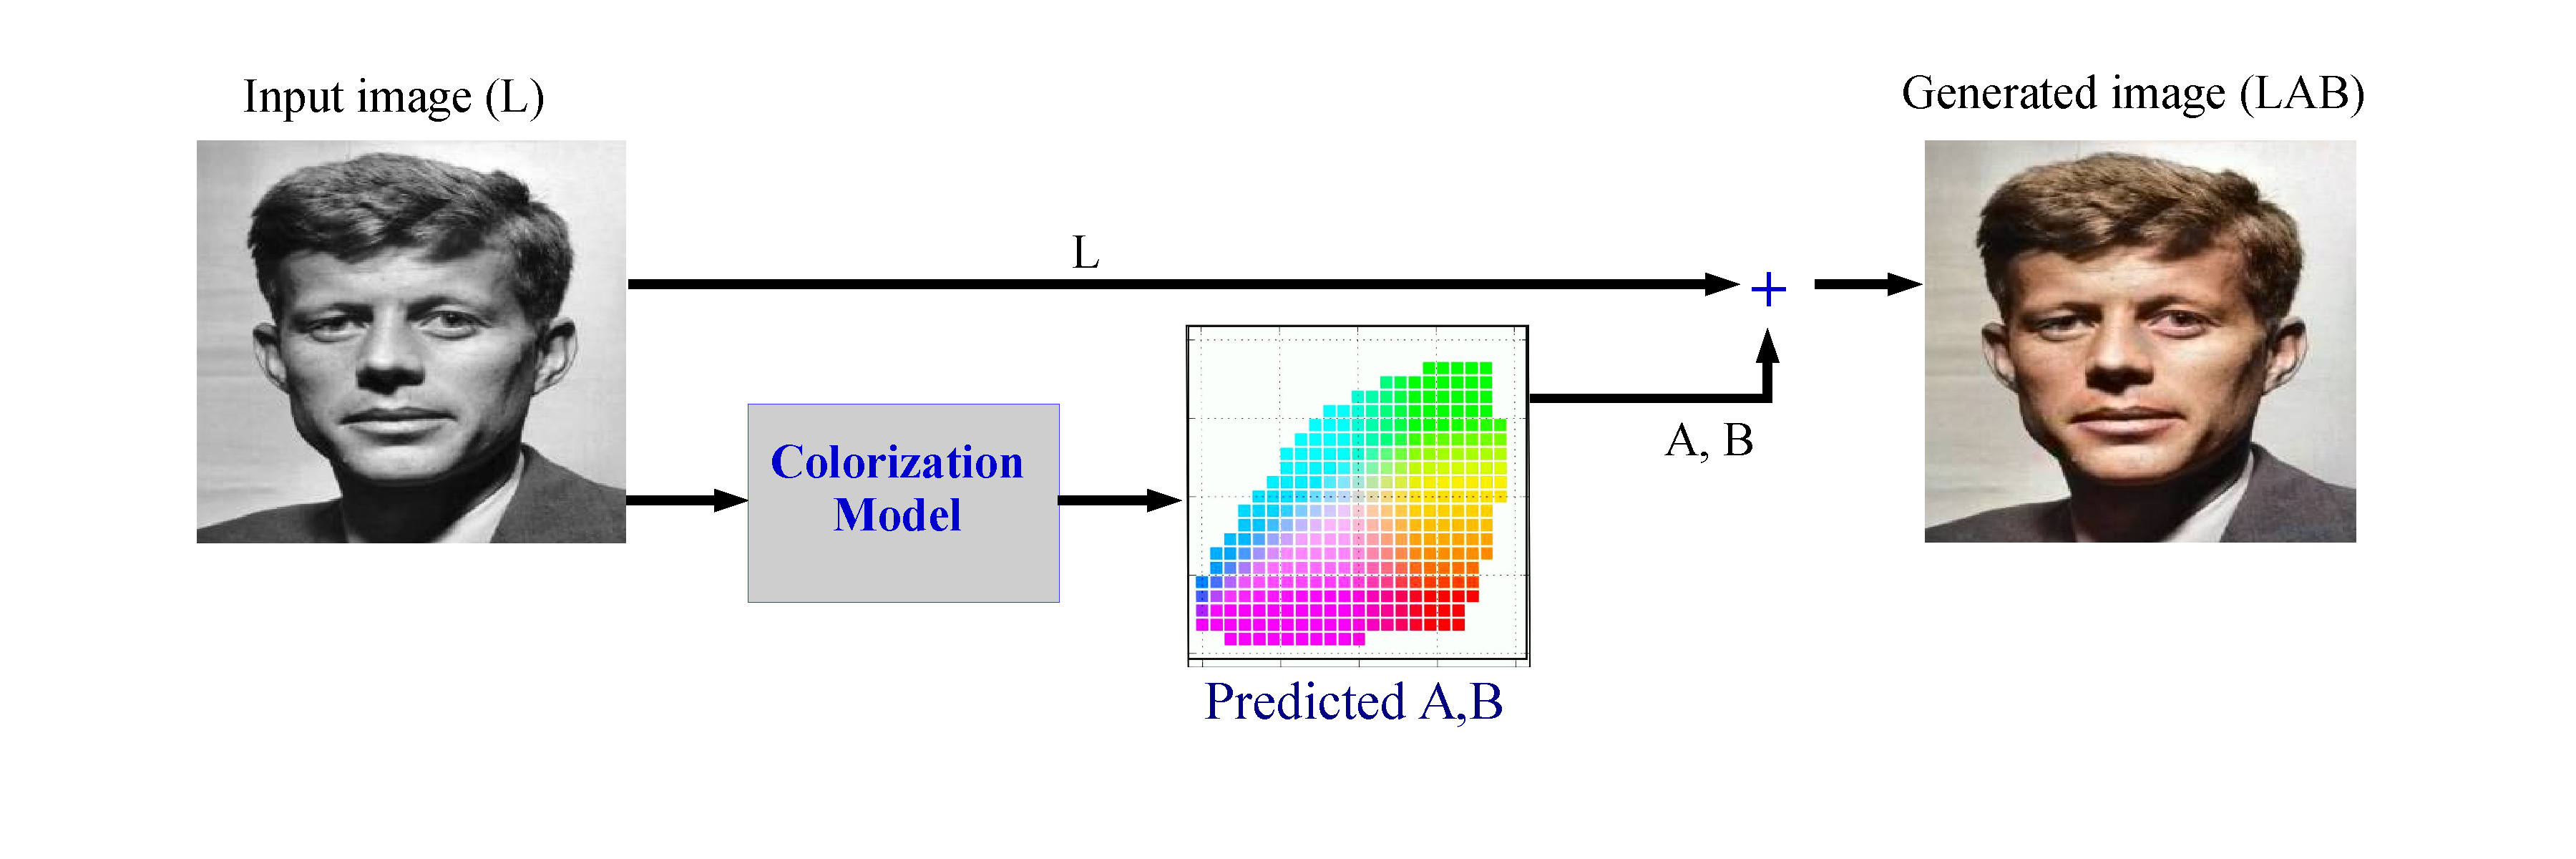
\includegraphics[width=\linewidth]{Figs/6.pdf}
\vspace{-13mm}
\caption{Basic image colorization procedure is shown. LAB color-space is generally used for convenience (\textit{i.e.}, one less unknown dimension); given the lightness channel $L$, task for the colorization model is to predict $A$ and $B$ channels so that the colorized image appears natural. }
\label{fig:col}
\end{figure}  

Colorizing a gray-scale image (\textit{i.e.}, only intensity values are known) is a difficult and ill-posed problem. Computer vision community have approached this problem in different ways over the last few decades \cite{zhang2016colorful, cheng2015deep, bugeau2014variational, charpiat2008automatic, luan2007natural, konushin2006interactive}. Before the advent of deep-learning \cite{lecun2015deep}, researchers have tried many classical techniques \cite{charpiat2008automatic, luan2007natural, konushin2006interactive, levin2004colorization, lagodzinski2008digital} to capture relationships between color components ($RGB$ or $LAB$) and image level features. 
Due to multi-modality and ill-posed nature of the problem, optimization based techniques \cite{levin2004colorization, charpiat2008automatic} and probabilistic models \cite{lagodzinski2008digital} were the only ones that achieved decent colorization performance in few specific applications. 
However, overall performance of these techniques, in general, were still poor due to the high non-linearity and abstract nature of color-feature relationship.  

Recently, deep-learning based image colorization techniques \cite{zhang2016colorful, cheng2015deep, varga2016fully, li2017watergan}, trained over millions of images, have shown significantly better performance over the earlier classical methods. For instance, the current state-of-the-art, `colorful colorization' \cite{zhang2016colorful}, can fool a human observer $32\%$ of the time in a \textit{colorization Turing-test} scenario. \textbf{Additionally,  how use of GANs are likely to improve the performance which why we are going to try?}

\textbf{In this project, we } 
// \textit{need to be added. need to be added. need to be added. need to be added. need to be added. need to be added. need to be added. need to be added.
need to be added. need to be added. need to be added. need to be added. need to be added. need to be added.
need to be added. need to be added. need to be added. need to be added. need to be added.}

\section{Background and Related Work}\label{sec:back}
As mentioned in the previous Section, image colorization is an ill-posed problem due to multi-modality and ambiguity. 
While some natural objects commonly hold the same color (e.g grass is \textit{usually} green), many are left up for interpretation. 
For example, given a gray-scale image of someone wearing a dark colored shirt, 
there is no way of figuring out the true color. 
Instead, the objective is to come up with a colorization that appears real, \textit{i.e.}, natural. 

User-based approaches \cite{levin2004colorization, konushin2006interactive, reinhard2001color, vrhel1992color} were popular for being fast and relatively accurate as user can provide a good prior for the inherent color distribution. However, these methods are not applicable for large scale automatic colorization, which led researchers to adopt optimization and probabilistic approaches \cite{charpiat2008automatic, bugeau2014variational, lagodzinski2008digital}. 
These approaches model a likelihood based color approximation for each pixel given the neighborhood information. 
Few methods introduce additional step for spatial coherency through image based segmentation as well. However, overall colorization performance of these approaches are not very appealing \cite{deshpande2015learning} for general usage in a large scale. This is because the prior distribution of color-space is domain-dependant; for instance, face images, underwater images, outdoor and satellite images, all have different color distributions. Besides, it is difficult to capture the highly non-linear and abstract color-feature relationships without large-scale training. 

In recent times, deep-learning based approaches \cite{zhang2016colorful, cheng2015deep, varga2016fully, li2017watergan} have produced significantly better colorization performance as they can extract highly non-linear spatial relationships if trained over large datasets. 
The convolutional layers learn appropriate filters to produce good feature-space representations from raw images. These feature extraction and filtering is performed over multiple layers 
to capture complex spatial relationships within the image-space, which is useful for image-to-image translation tasks. \textbf{Additionally,  Prospects of GANs GANs .......}

\textbf{In this project, we } 
// \textit{need to be added. need to be added. need to be added. need to be added. need to be added. need to be added. need to be added. need to be added.
need to be added. need to be added. need to be added. need to be added. need to be added. need to be added.
need to be added. need to be added. need to be added. need to be added. need to be added.}  

\section{Generative Approaches}
In our project, we tried two classical methods: \textit{colorization using optimization} \cite{levin2004colorization}, \textit{colorization via multimodal predictions} \cite{charpiat2008automatic}. The former is not an automatic approach (user provides color distribution prior), whereas, the later uses a set of reference images to formulate color distribution. Their operations are discussed in our term report; this paper focuses on the third generative approach, \textit{colorful image colorization} \cite{zhang2016colorful}, which is adopted in our project. 

\subsection{\textbf{Adopted Model: Colorful Image Colorization}}
Colorful image colorization \cite{zhang2016colorful} is considered as a major breakthrough on this problem. Published on 2016, it has managed to set a new benchmark for performance. It is an automatic approach that produces realistic colorizations based on a CNN-based model. 
It poses the problem as a multi-modal classification problem. The objective function is carefully designed to map the image-to-image translation problem to a classification problem. First, it takes advantage of the fact that $A$, $B$ color components of LAB colorspace for natural images are concentrated in a small region, which are discretized into finite number of bins ($Q$). 
Given the lightness channel ($L_p$) of a pixel $p$, its $A$, $B$ pair corresponds to a particular bin (out of $313$ bins in total), which is mapped to a 1-hot vector ($Z_p$). 
Consequently, task of the classification model, is to predict which bin each pixel corresponds to. That is, the output is a $313$-mode probability distribution ($ \hat{Z_p}$) for each pixel $p$. The objective function is modelled as a cross entropy loss between $Z$ and $\hat{Z}$, expressed as follows: 

\[ L_{col}(Z, \hat{Z}) = - \sum_p Z_p \sum_{q \in Q} Z_p[q] log(\hat{Z_p}[q])   \] 

This cross-entropy loss is further augmented with class rebalancing, to encourage rare colors. The detailed model specification, as shown in Fig. \ref{fig:col_main}, is an 8-layer CNN architecture where each conv layer refers to a block of $2$ or $3$ repeated
conv and ReLU layers \cite{nair2010rectified}, followed by a BatchNorm layer \cite{ioffe2015batch}. The network has no pool layers; 
all changes in resolution are achieved through spatial down-sampling or up-sampling between conv blocks.


\begin{figure}[h]
\centering
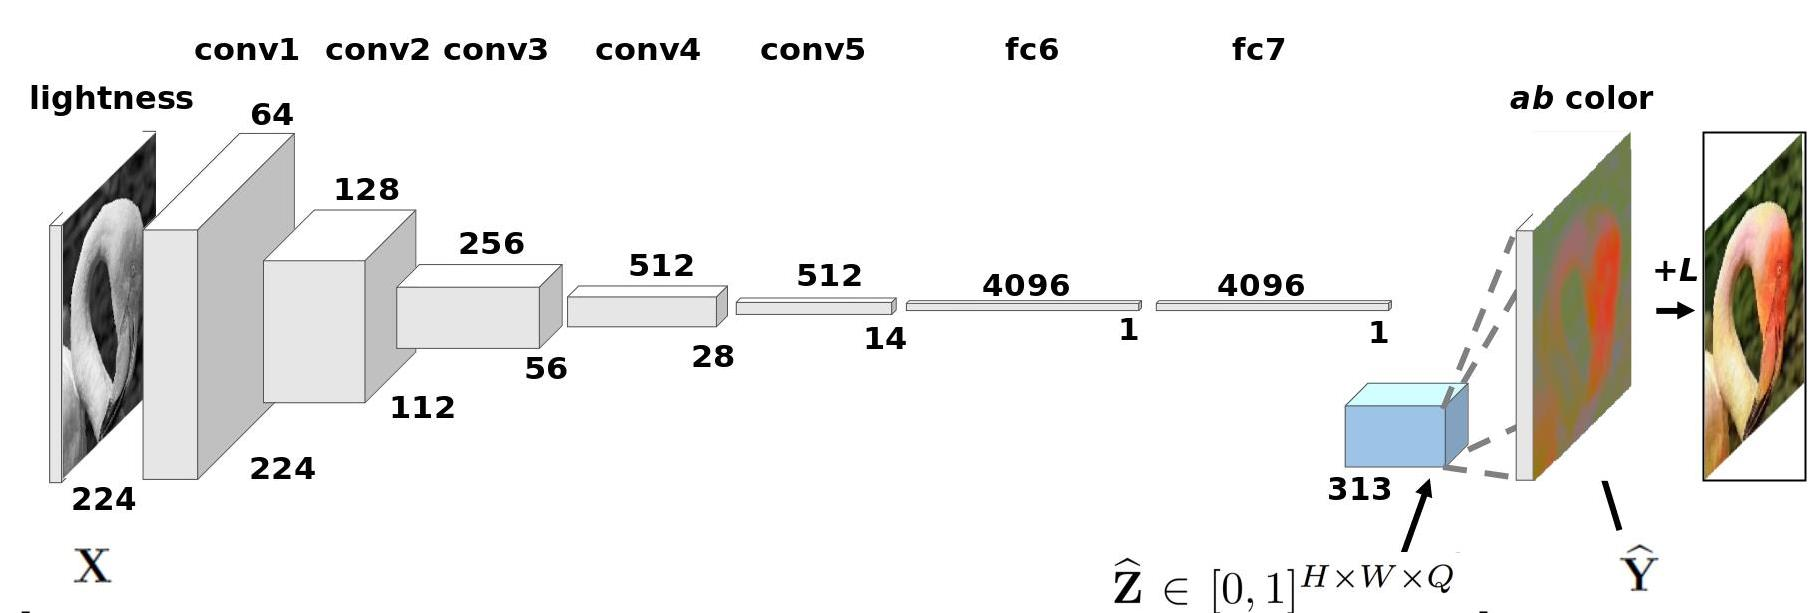
\includegraphics[width=0.8 \linewidth]{Figs/one.jpg} 
\caption{Architecture of colorful image colorization model \cite{zhang2016colorful} that is adopted in our evaluation}
\label{fig:col_main}
\end{figure}  


\begin{figure}[!h]
\centering
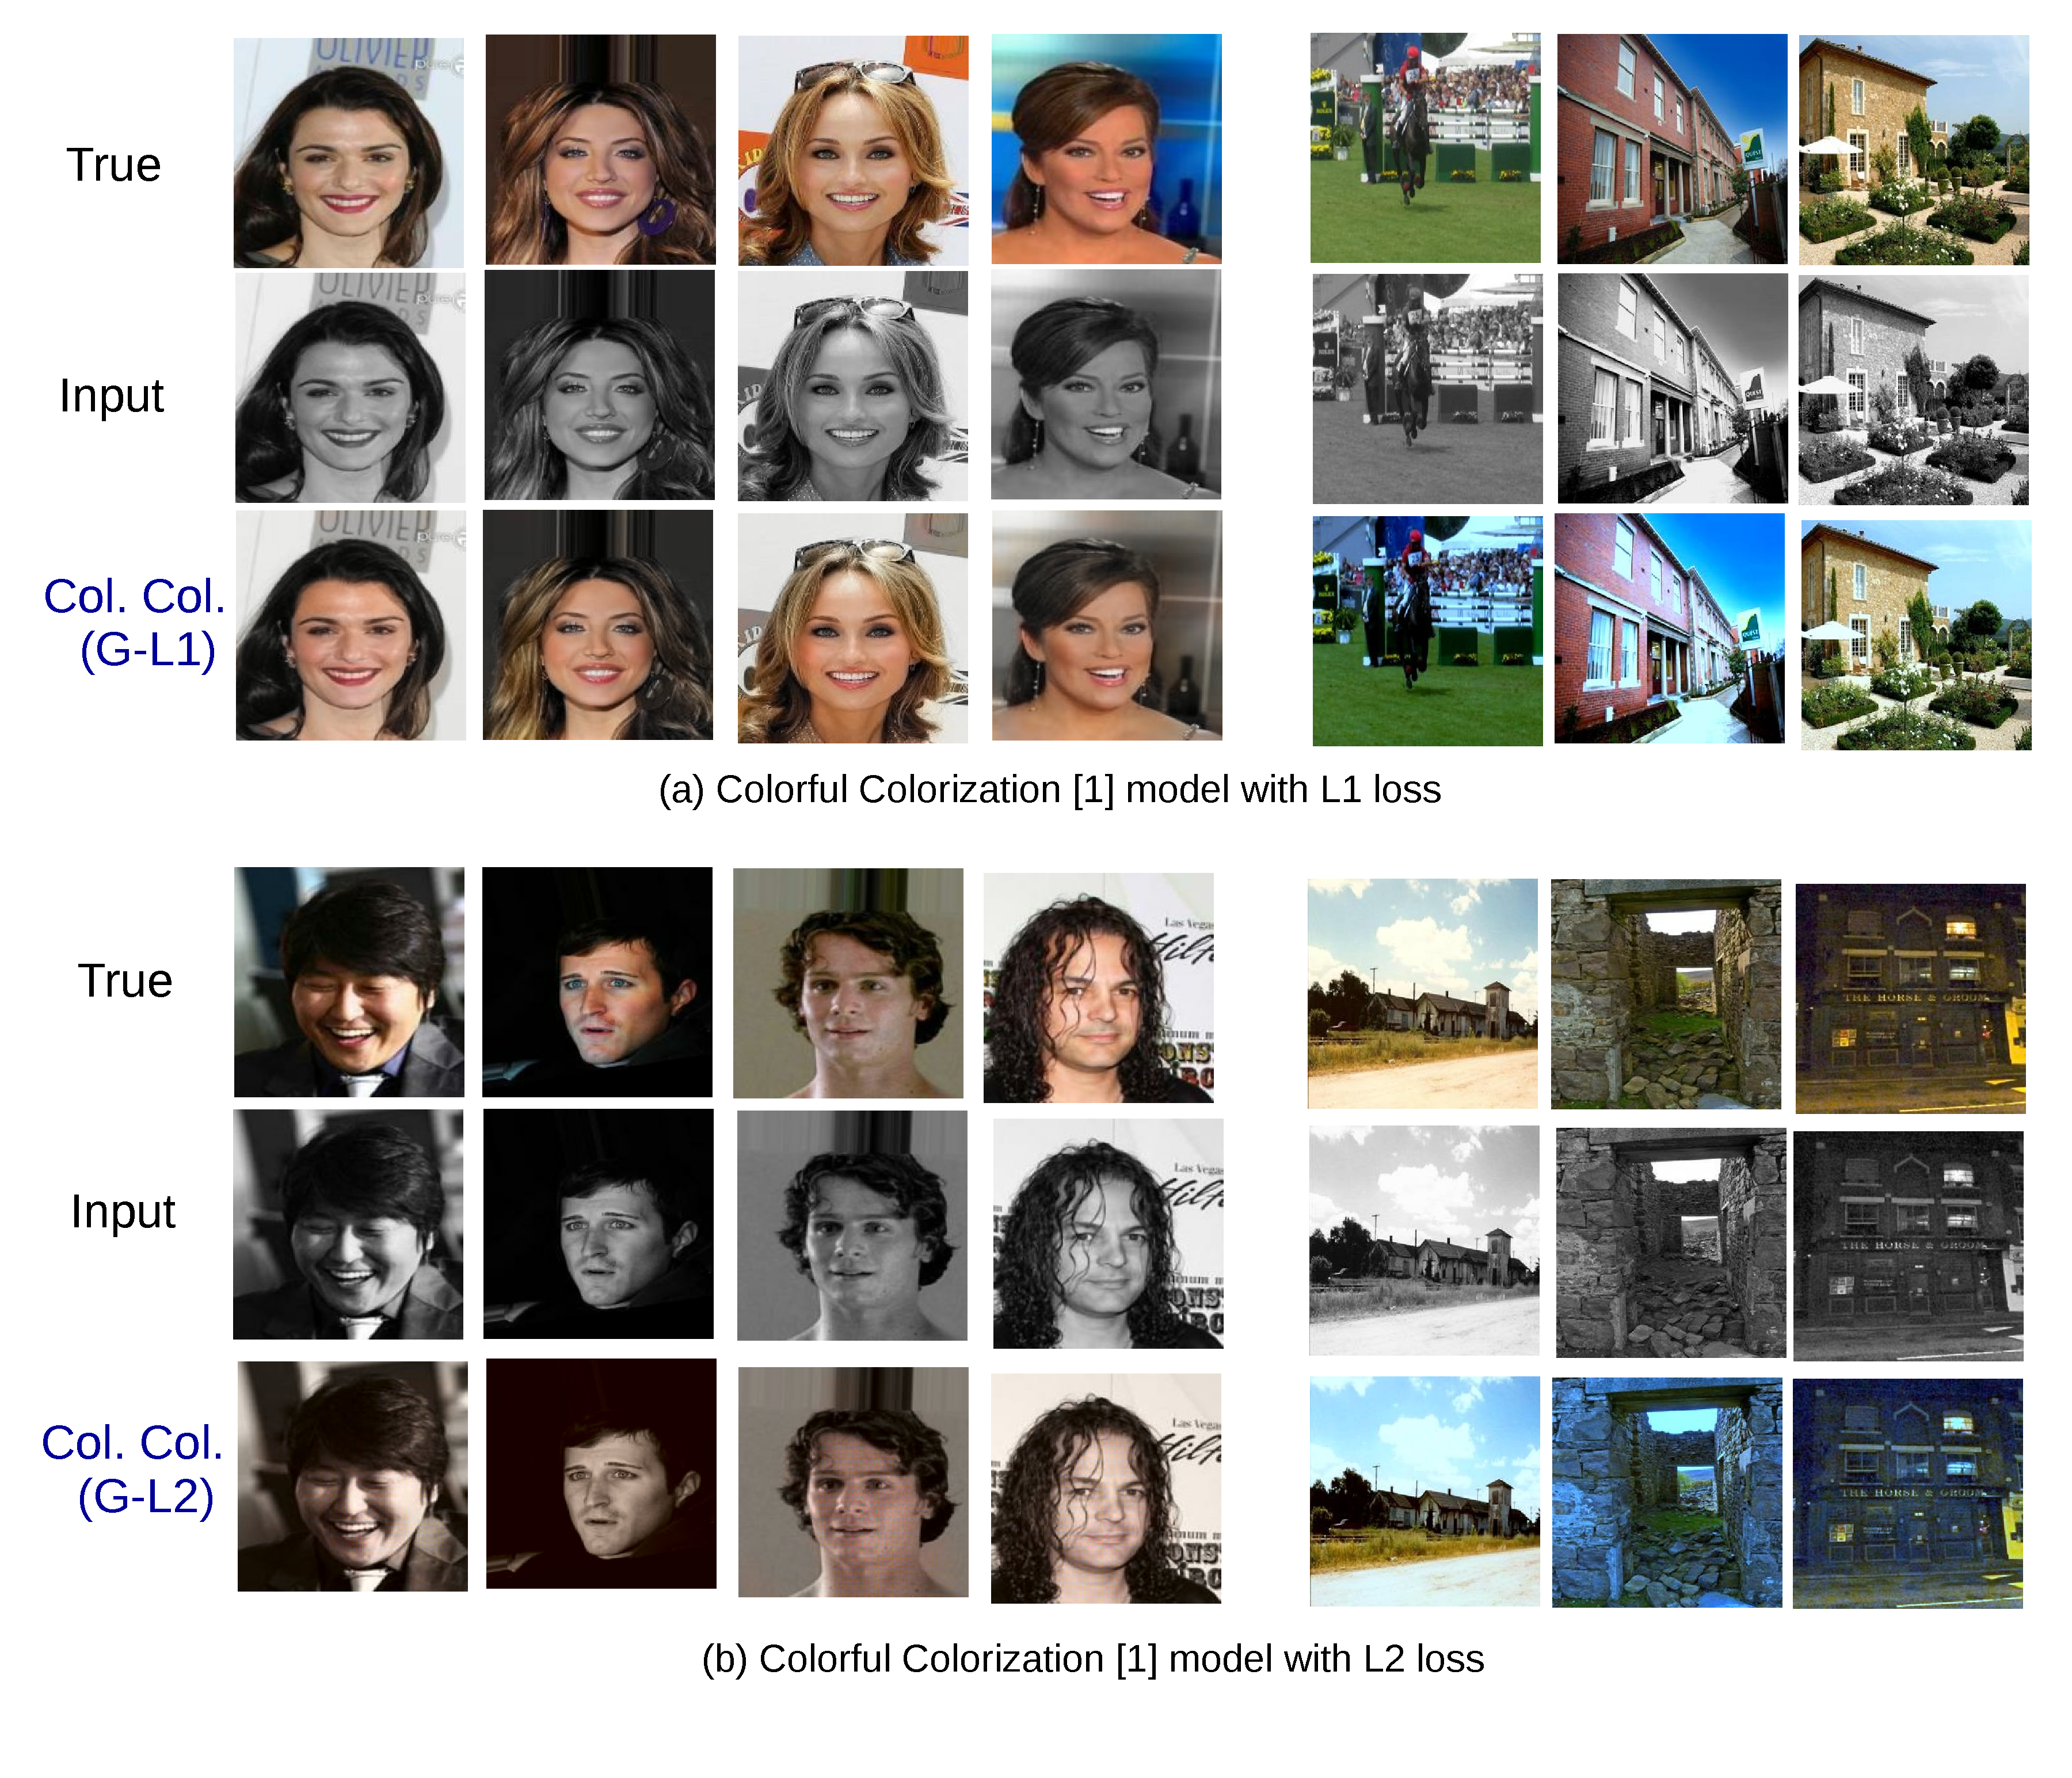
\includegraphics[width=0.8 \linewidth]{Figs/4.pdf} 
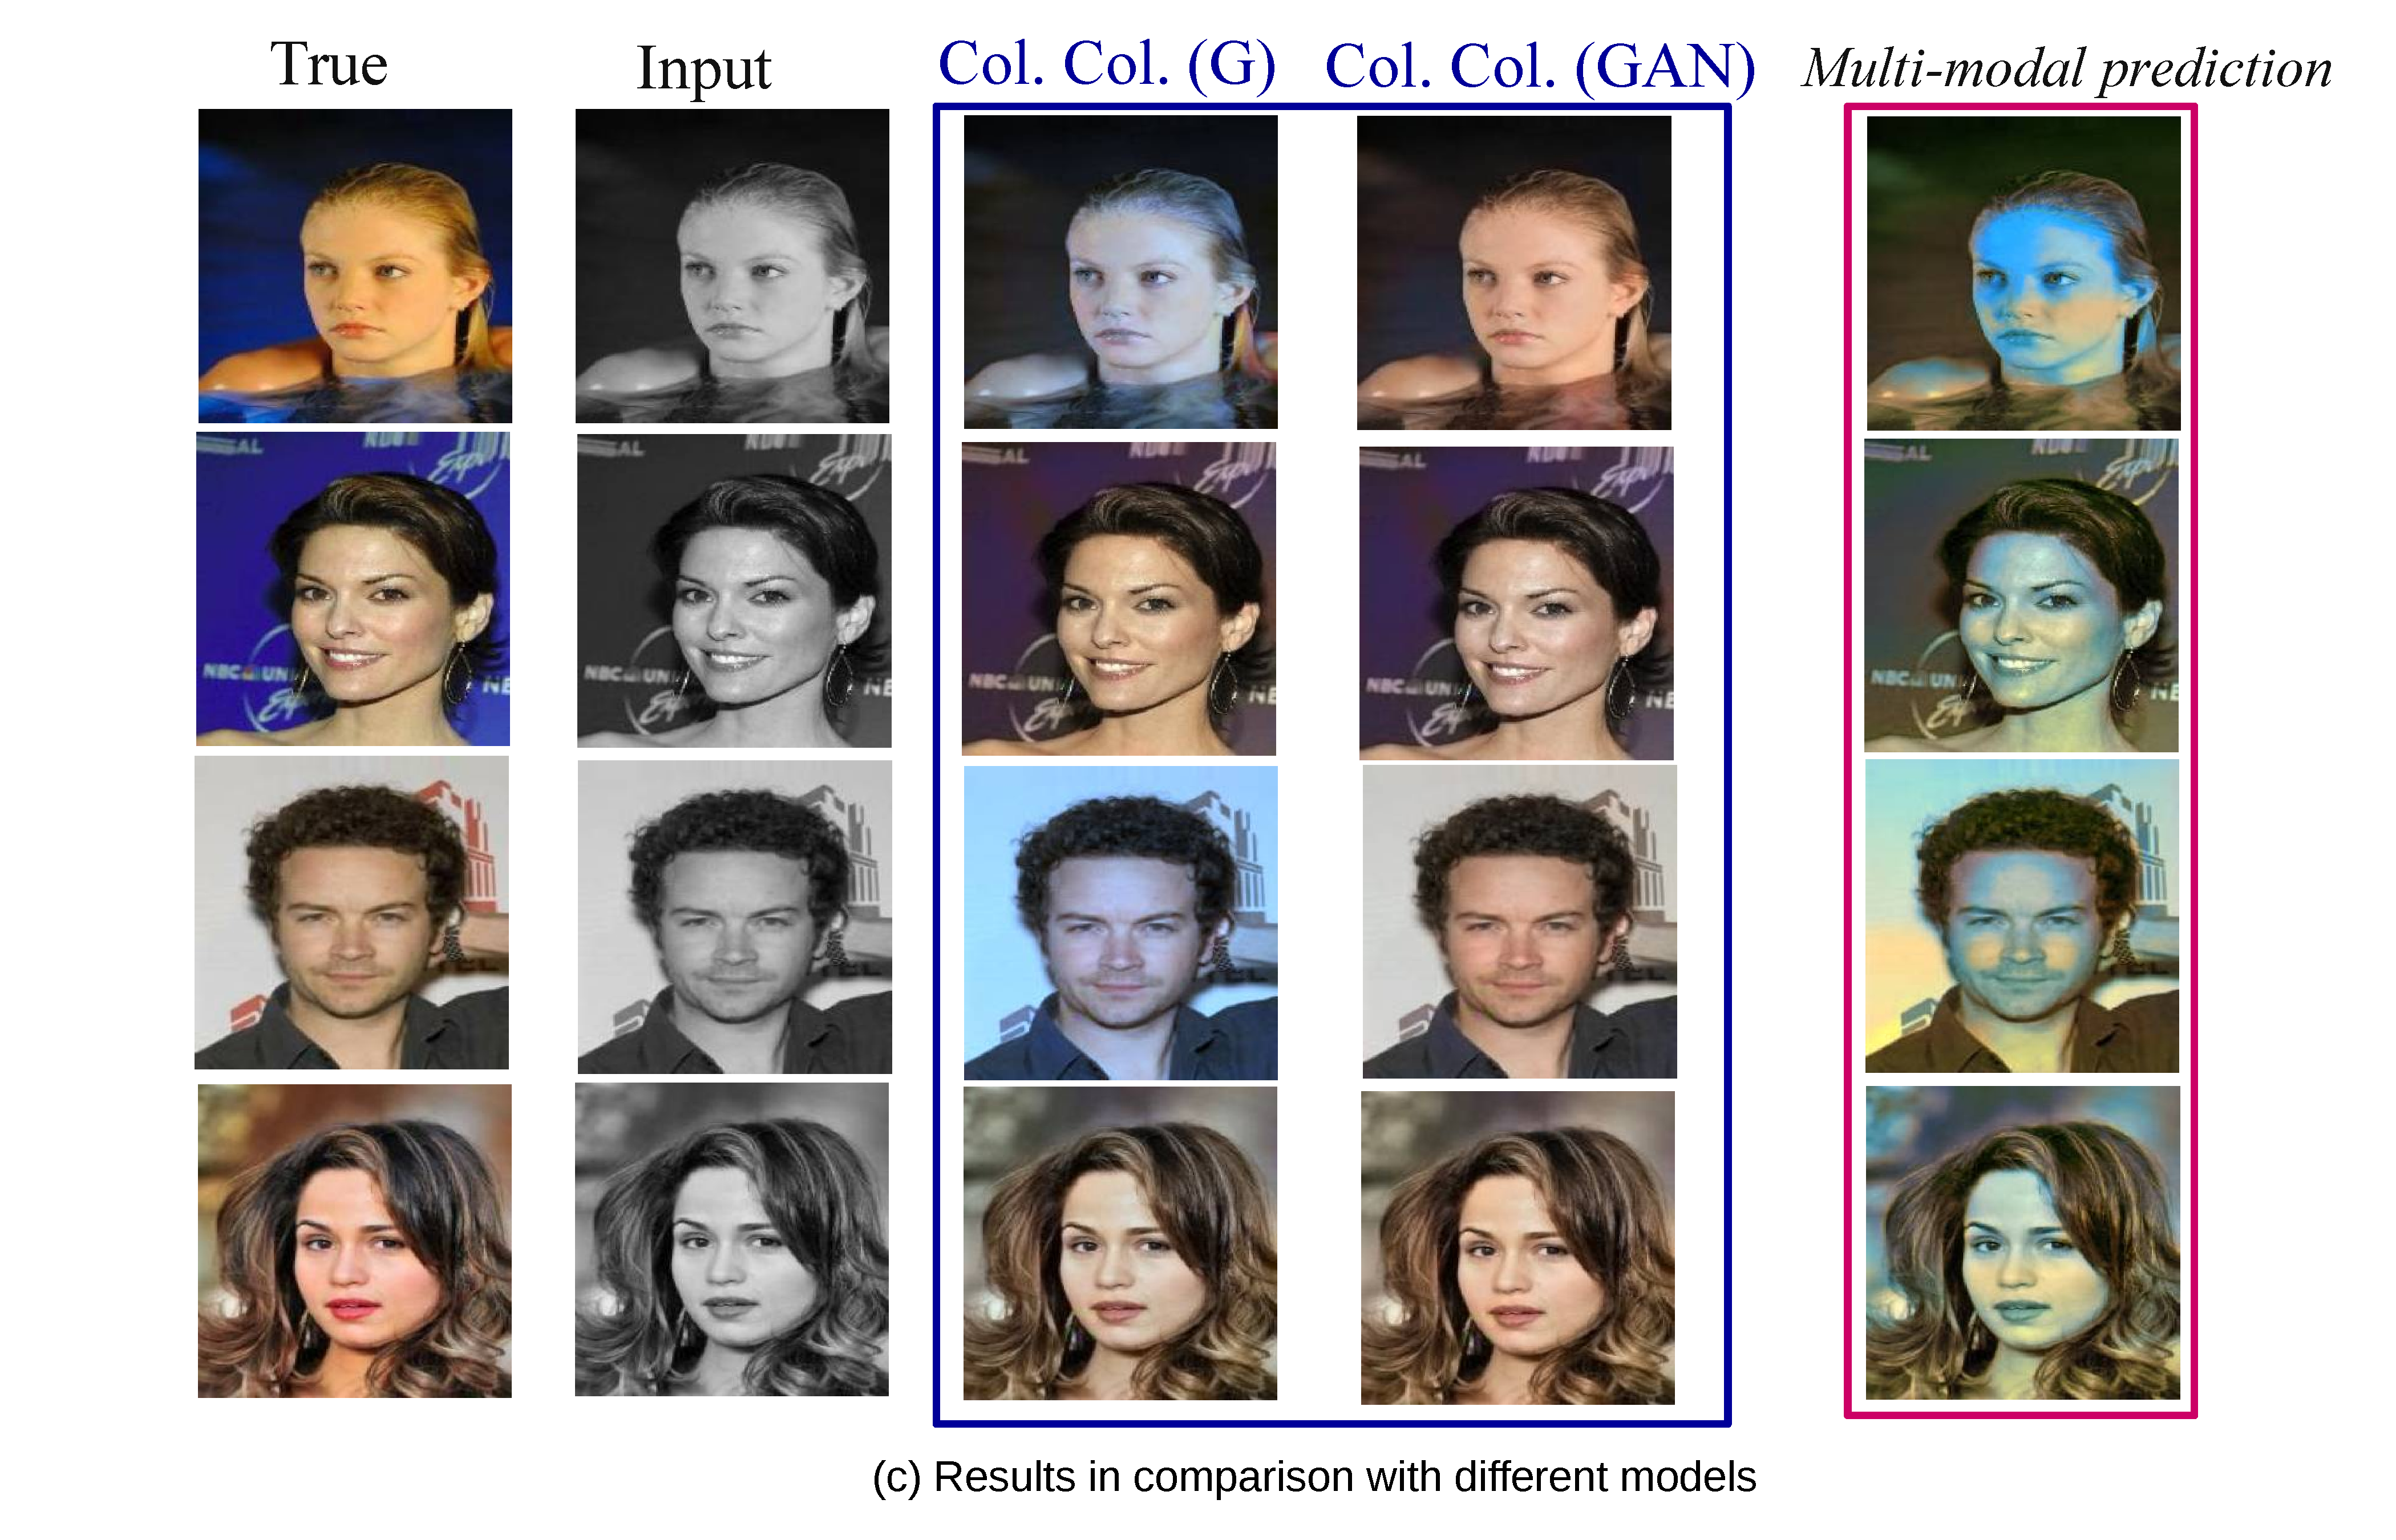
\includegraphics[width=0.7 \linewidth]{Figs/82.pdf}
\vspace{-1mm}
\caption{Results for the colorful colorization model \cite{zhang2016colorful} with (a) L1 and (b) L2 loss is shown; First $4$ columns show few examples from the test set of CelebA \cite{celebA} dataset, while the rest ($3$) columns correspond to Places2 \cite{places2} dataset. Comparison for colorful colorization model used as a generator only (Col. Col. (G)), and as a generator in a GAN (Col. Col. (GAN)), is shown in (c); also, results obtained by colorization via multi-modal prediction \cite{charpiat2008automatic} is provided in the last column to demonstrate the degree of improvements using colorful colorization model.}
%\vspace{-20mm}
\label{fig:res_full}
\end{figure}  


\subsection{\textbf{Implementation Details and Model Changes}}
While working on designing a generator for our GAN-based model, we investigated this model with different objective functions ($L_1$ loss, $L_2$ loss, least-squared loss, etc.) instead of their cross-entropy based loss function. This is due to the fact that in a GAN-based model, \textit{discriminator} expects an image from the \textit{generator}, 
and tries to discriminate it as real or fake in order to force the generator to get better.  
Therefore, rather than adopting their classification model directly, we implemented their architecture 
using objective functions based on $L_1$, $L_2$, least-squared loss (so that it outputs an image, not classification probabilities). Additionally, it made our model end-to-end trainable, which can be easily incorporated in a GAN-based architecture. 

Given an input image $I$, the network is fed with its $L$ channel ($I_L$); the output layer of the network is adjusted to predict $\hat{I}_{AB}$. We have found $L_1$ and $L_2$ loss functions perform quite well with this model. These loss functions between true $I_{AB}$ and $\hat{I}_{AB}$ can be expressed as follows:

\[ L_1 (I_{AB}, \hat{I}_{AB}) = \lambda \sum_p | I_{AB}[p] - \hat{I}_{AB}[p] | \]  
\[ L_2 (I_{AB}, \hat{I}_{AB}) = \lambda \sum_p ( I_{AB}[p] - \hat{I}_{AB}[p] )^2 \]  

Here, $\lambda$ is a normalization constant. CelebA datasets \cite{celebA} is used for training primarily, that has $195K$ training examples (a total of  $202K$ images); 
In a separate training, a set of $200K$ images from Places2 dataset \cite{places2} were also used for training\footnote{Larger datasets like ImageNet \cite{deng2009imagenet} and full Places2 challenge dataset were not used for the project due to time constraint; however, we are planning to train our final GAN-based model over these datasets during the summer.}. Training was performed using two $1080$ gpus (in a core-i7 machine having $64$GB RAM); training time for $100K$ iterations with a batch size $32$ was about $2$-$3$ days for each trial. The implementation is done using TensoFlow \cite{abadi2016tensorflow} in python.    

\subsection{\textbf{Results}}
We found that this model performs better with $L_1$ loss function compared to $L_2$ loss. This might be because of the averaging effect of $2$-norm which causes a blurry colorization (similar phenomena is discussed in \cite{zhang2016colorful}). The results on few test cases are shown in Fig. \ref{fig:res_full}. 

In the results state above, colorful colorization model is used as a generator only (\textbf{Col. Col. (G)}); we also used this model as a generator in a GAN (\textbf{Col. Col. (GAN)}) to investigate its performance. As illustrated in Fig. \ref{fig:res_full}(c), images colorized  by Col. Col. (GAN) are more realistic and consistent than Col. Col. (G). In addition, we provided results obtained by colorization via multi-modal prediction \cite{charpiat2008automatic} to demonstrate the degree of improvements using colorful colorization model. 

The colorful colorization model, as a generator alone, and as a generator in a GAN, achieve decent colorization performance. Next, we discuss other GAN based models for image colorization, which we investigated in our project. 
 

 

\section{Adversarial Approaches}
Generative Adversarial Networks (GANs) [REF] are a recent class of generative models based on game theory
in which a generator network is pitted against an adversary. The adversary or discriminator, $D$, is a 
neural network trained to discriminate between real samples and samples generated by the generator. The
generator, $G$, is trained to fool the adversary. They have shown very impressive results towards
various tasks including inpainting, domain adaptation, and image colorization. Due to the difficulty in
training them in practice, there have been several theoretical approaches towards stabalizing their training
by providing better gradients for the generator in terms of changing the loss function for the discriminator.
Regular GANs modeled the discriminator as a classifier with the sigmoid cross entropy loss function,
which has been shown to suffer from the vanishing gradient problem [REF]. We experimented with four different
variations of GANs: Regular GANs, Least Squares GANs (LSGAN), Energy-Based GANs (EBGAN), and Wasserstein GAN
(WGAN). There has been little work in using GANs for the task of image colorization. Most notable is the
Pix2Pix model which uses the normal GANs loss, but also show that often their generator fails to generate
any color at all. We hypothesize that in comparison to the common task in which GANs are trained to generate
an image from a noise prior, the discriminator for the task of colorization has a much more difficult job
due to the visual similarity between images. For this reason, a much stronger discriminator is needed, but
as shown in [REF], with the normal GANs loss, as the discriminator gets better, the gradients passed to the
generator, and therefore the generator itself, become worse. For this reason we chose to explore other
options for the discriminator loss. Our model is set up as a \textit{conditional} GAN (cGAN), in which the
generator is conditioned on the grayscale image. The rest of this section compares the different GAN
formulations, and ends with our architecture designs. We combine the GAN objective with $L_1$ and $L_2$ in
order to provide some sense of ground truth. These can be expressed as:

\[ \mathcal{L}_{L_1}(G) = \mathbb{E}_{x,y\sim p_{data}(x,y)}[||y-G(x)||_1] \]
\[ \mathcal{L}_{L_2}(G) = \mathbb{E}_{x,y\sim p_{data}(x,y)}[(y-G(x))^2] \]


\noindent These are able to capture low frequencies, but have been shown to lack in capturing high
frequencies, resulting in blurry images in the case of autoencoders, or saturated colors in the case of
colorization. These imperfections should in theory be rejected by the discriminator, which results in
successfully capturing high frequencies in images such as sharp edges and bright colors. Note that using
these losses along with the GAN loss does not change the discriminator's objective, it is the generator
that is required to fool the discriminator as well as be near the ground truth.

\subsection{DCGANs}
Because of the high dimensionality and spacial structure of images, we chose to use Deep Convolutional GANs
(DCGANs), which take advantage of the recent successes of Convolutional Neural Networks (CNN) as part of
their architecture, as opposed to the simple neural networks used in [GAN PAPER]. The objective function is
given as:

\[\min\limits_{G}\max\limits_{D} \mathbb{E}_{x \sim p_{data(x)}} [logD(\textbf{\textit{x}})] + \mathbb{E}_{z \sim p_z(z)}[log(1 - D(G(z)))]\]

\noindent where $p_{data}$ represents the true data, and $p_z$ represents some noise prior, e.g.
$z \sim \mathcal{N}$. 
for our conditional DCGAN can be expressed as:

\[ \mathcal{L}_{DCGAN}(G,D) = \mathbb{E}_{x,y \sim p_{data}} log D(x,y) + \mathbb{E}_{x \sim p_{data}}
log (1-D(x, G(x)))\]

\noindent where $x$ represents the grayscale image, and $y$ represents the $ab$ color values associated with
$x$. Combining this with our $L_1$ and $L_2$ loss functions gives us our final objective:

\[ G^* = \lambda_1 \mathcal{L}_{DCGAN} + \lambda_2 \mathcal{L}_{L_1} + \lambda_3 \mathcal{L}_{L_2} \]

\noindent where $\lambda_1$, $\lambda_2$, and $\lambda_3$ are hyperparameters. One should note that $z$
is discarded in this formulation, resulting in a deterministic model. Because of the high volume of information
given in the grayscale image in comparison to something like
conditioning on a class label, we believe the model would simply learn to discard $z$ as noise
(because that's quite literally what it is). Instead, we provide noise in the form of droupout in the
generator, but have not seen much difference in the output. We evaluated our method on the CelebA
dataset. Some results can be seen in Figure X. 

%\begin{figure}[h]
   %\centering
   %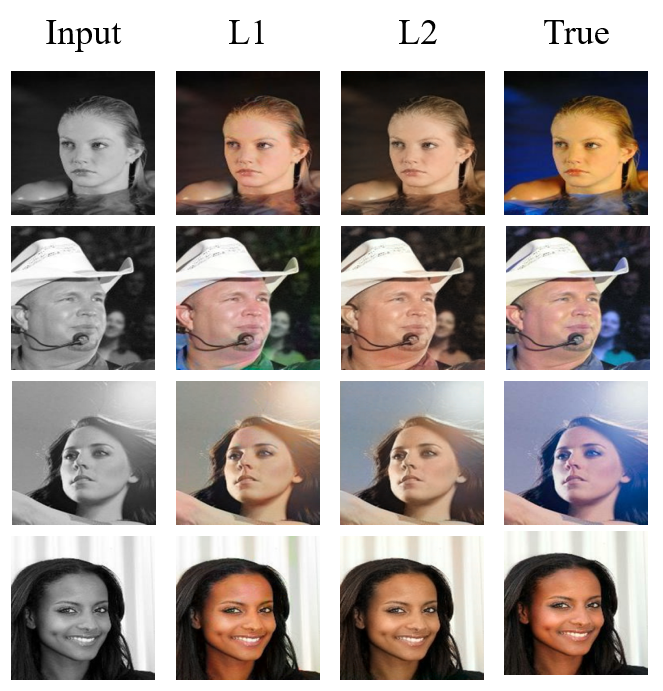
\includegraphics[width=0.8]{dcgan_results} 
   %\caption{Results of DCGANs evaluated on CelebA}
%\end{figure}  

\subsection{LSGANs}
Least Squares GANs (LSGANs) provide a least squares loss for the discriminator in order to penalize samples
that may have fooled the discriminator but do not lie close to the true data distribution. The objectives
for conditional LSGANs are defined as:

\[\min\limits_{D} V_{cLSGAN}(D) = \frac{1}{2} \mathbb{E}_{x,y \sim p_{data(x,y)}} [(D(x,y)-b) ^2] +
\frac{1}{2} \mathbb{E}_{x \sim p_{data}}[(D(G(x)) - a)^2] \]

\[\min\limits_{G} V_{cLSGAN}(G) = \frac{1}{2} \mathbb{E}_{x \sim p_{data(x)}} [(D(G(x))-c)^2] \]

\noindent where $a=0$ to denote the fake data, $b=1$ to denote the true data, and $c=1$ in order to try and
fool $D$. 

\noindent where $p_{data}$ represents the true data, $x$ represents the grayscale image, $y$ represents
the corresponding $ab$ color channels for $x$. 
We combine the LSGAN objective with $L_1$ and $L_2$ to give our final objective:

\[ G^* = \lambda_1 V_{cLSGAN} + \lambda_2 \mathcal{L}_{L_1} + \lambda_3 \mathcal{L}_{L_2} \]

\noindent where $\lambda_1$, $\lambda_2$, and $\lambda_3$ are hyperparameters. We evaluated LSGANs on
the CelebA dataset. Some results can be seen in Figure X.

%\begin{figure}[h]
   %\centering
   %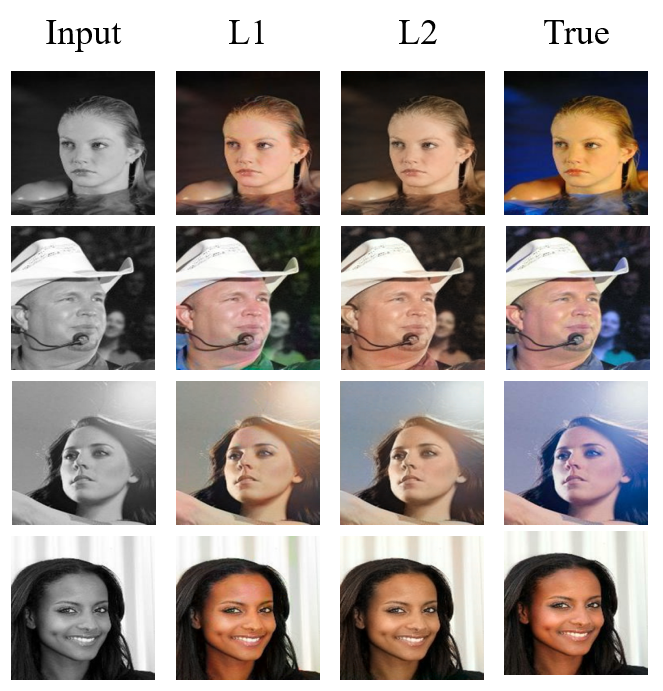
\includegraphics[width=0.8]{dcgan_results} 
   %\caption{Results of DCGANs evaluated on CelebA}
   %\label{fi}
%\end{figure}  

\subsection{EBGANs}
Energy-Based GANs (EBGANs) model the discriminator as an energy function that attributes low energies to
the regions near the data manifold and higher energies to other regions. Unlike the other GAN variations
mentioned, the EBGANs discriminator is modeled as an autoencoder, which aims to provide a more diverse
set of outputs as opposed to the binary logistic loss. 
The objectives for conditional EBGANs are defined as:

\[\mathcal{L}_{cEBGAN} D(x,y) = D(x,y) + max(0, (m-D(G(z)))) \]
\[\mathcal{L}_{cEBGAN} G(x) = D(G(x)) \]


\noindent where $m$ is some margin, $x$ represents the grayscale image, $y$ represents the corresponding
$ab$ color channels for $x$. We combine the EBGAN objective with $L_1$ and $L_2$ to give our final objective:

\[ G^* = \lambda_1 \mathcal{L}_{cEBGAN} + \lambda_2 \mathcal{L}_{L_1} + \lambda_3 \mathcal{L}_{L_2} \]

\noindent where $\lambda_1$, $\lambda_2$, and $\lambda_3$ are hyperparameters. We evaluated EBGANs on
the CelebA dataset. Some results can be seen in Figure X. 

\subsection{WGAN}
The Wasserstein GAN (WGAN) approximates the Earth Mover (EM) distance given a set of $K$-Lipschitz functions 
$f$. In order to have the parameters $w$ lie in a compact space and ensure $f$ is $K$-Lipschitz, the weights
of the network are clamped to some range. Because the EM distance is continuous and differentiable, the
discriminator (critic) should be trained to optimality, which offers better gradients to the generator. This 
offers stable training at the expense of slow training, because the critic must be updated multiple times
for one update of the generator. Our conditional WGAN objective function is:

\[\mathcal{L}_{cWGAN} = \max\limits_{w \in W} \mathbb{E}_{x,y \sim \mathbb{P}_{data}}[f_w(x,y)] -
\mathbb{E}_{x \sim p_{data}}[f_w(G(x))]\]

\noindent where $x$ represents the grayscale image and $y$ represents the corresponding
$ab$ color channels for $x$. We combine the WGAN objective with $L_1$ and $L_2$ to give our final objective:


\[ G^* = \lambda_1 \mathcal{L}_{cWGAN} + \lambda_2 \mathcal{L}_{L_1} + \lambda_3 \mathcal{L}_{L_2} \]

\noindent where $\lambda_1$, $\lambda_2$, and $\lambda_3$ are hyperparameters. We evaluated WGAN on
the CelebA dataset. Some results can be seen in Figure X. 

%\begin{figure}[h]
   %\centering
   %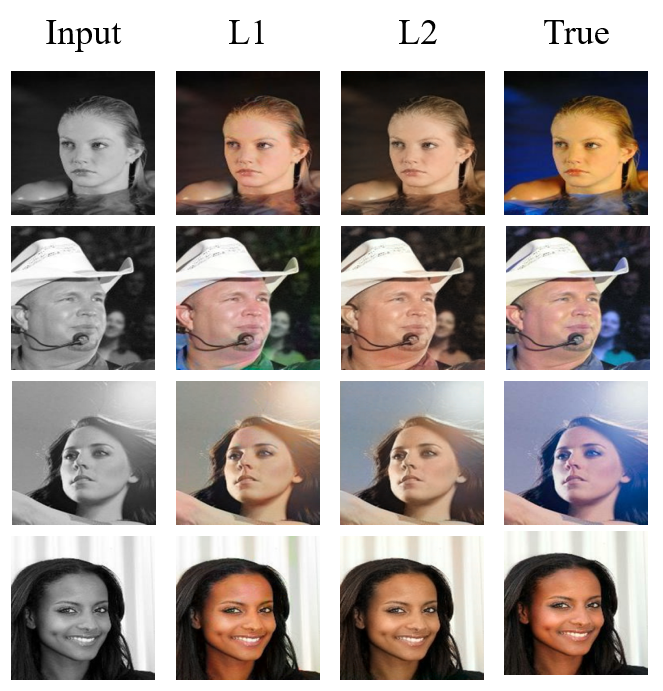
\includegraphics[width=0.8]{dcgan_results} 
   %\caption{Results of DCGANs evaluated on CelebA}
   %\label{fi}
%\end{figure}  


\section{Conclusion}
Conclusion

\vspace{1mm}
\bibliographystyle{unsrt}
\footnotesize
\bibliography{cvbibs}

\end{document}
